\documentclass[11pt]{article}
%Gummi|065|=)

\usepackage{eurosym}
\usepackage{listings}
\usepackage{color}
\usepackage{graphicx}
\graphicspath{ {.} }
\usepackage{upgreek}
\usepackage{titlesec}

%for code snippets
\lstset{
  language=C,                % choose the language of the code
  %numbers=left,                   % where to put the line-numbers
  stepnumber=1,                   % the step between two line-numbers.        
  numbersep=5pt,                  % how far the line-numbers are from the code
  backgroundcolor=\color{white},  % choose the background color. You must add \usepackage{color}
  showspaces=false,               % show spaces adding particular underscores
  showstringspaces=false,         % underline spaces within strings
  showtabs=false,                 % show tabs within strings adding particular underscores
  tabsize=2,                      % sets default tabsize to 2 spaces
  captionpos=b,                   % sets the caption-position to bottom
  breaklines=true,                % sets automatic line breaking
  breakatwhitespace=true,         % sets if automatic breaks should only happen at whitespace
  title=\lstname,                 % show the filename of files included with \
}

\setcounter{secnumdepth}{4}

\titleformat{\paragraph}
{\normalfont\normalsize\bfseries}{\theparagraph}{1em}{}
\titlespacing*{\paragraph}
{0pt}{3.25ex plus 1ex minus .2ex}{1.5ex plus .2ex}


\title{\textbf{Home Aquaponics System}}

\author{Samuel Schober, Konrad Kelc\\
		Matthias Schwebler, Ramin Bahadoorifar\\}
\date{}

\begin{document}

\maketitle
\begin{titlepage}
    \begin{center}
        \vspace*{1cm}
		\title{\textbf{Home Aquaponics System}}

        \vspace{2.5cm}

        2016 - 5BHIT

        \vspace*{5mm}

        \small{Samuel Schober, Konrad Kelc\\Matthias Schwebler, Ramin Bahadoorifar}

        \vspace*{2cm}

        \vfill

        \begin{center}
        \end{center}

    \end{center}
\end{titlepage}

\section{Einf\"uhrung}
Aquaponik ist ein Verfahren, welches die Aufzucht von Fischen mit der Aufzucht von Nutzpflanzen verbindet. Im Wesentlichen handelt es sich dabei um einen geschlossenen Wasserkreislauf, in dem die entsprechenden N\"ahrstoffe „automatisch“ erzeugt werden; d.h. die Ausscheidungen der Fische werden durch Bakterien in N\"ahrstoffe f\"ur die Pflanzen umgewandelt. Es soll eine vollautomatisierte L\"osung f\"ur ein Aquaponik-System f\"ur kleine Haushalte als Prototyp geschaffen werden. Diese beinhaltet einerseits eine geeignete Konstruktion die sowohl das Aquarium enth\"alt als auch die ent-sprechende \"Uberwachung und Regelung des Systems.


\section{Projektdaten}

\subsection{Projetkteam}
Name: Samuel Schober \\
E-Mail: sschober@student.tgm.ac.at \\
\\Name: Matthias Schwebler \\
E-Mail: mschwebler@student.tgm.ac.at \\
\\Name: Ramin Bahadoorifar \\
E-Mail: rbahadoorifar@student.tgm.ac.at \\
\\Name: Konrad Kelc \\
E-Mail: kkelc@student.tgm.ac.at

\subsection{Projektbeschreibung}
Im Rahmen des Projekts wird ein Tool zur \"Uberwachung und Steuerung von Metadaten eines Aquaponic Systems, entwickelt und mit entsprechender Hardware realisiert. Dabei werden Sensoren von einem Raspbery Pi angesprochen und die Ergebnisse lokal gespeichert, welche sp\"ater \"uber eine Webseite eingesehen werden k\"onnen (M\"ogliche Methoden der \"Ubertragung werden im Kapitel X.x erleutert - TODO). Des Weiteren kann der Benutzer \"uber die Weboberfl\"ache die Wassertemperatur sowie die Belichtungsdauer der Pflanzen regeln. Zus\"atzlich erh\"alt der Benutzer Vorschl\"age f\"ur einen sinnvollen Besatz des Aquariums sowie f\"ur die Pflanzenwahl und deren Bed\"urfnisse.

\section{Voruntersuchung des Projekts}
\subsection{Ist-Erhebung}
Aquaponic Systeme sind haupts\"achlich im gr\"o{\ss}eren Ma{\ss}stab bei der Aufzucht von Nutzpflanzen im Einsatz. F\"ur den normalen Haushalt gibt es allerdings bis jetzt keine Marktf\"ahige L\"osung. Die gr\"o{\ss}ten zwei Crowdfunding Projekte sind:
\begin{itemize}
	\item \textbf{EcoQube C}\\
		Der EcoQube C vereint ein Handliches Aquaponics System mit elegantem Design, jedoch mangelt es an Konfigurierbarkeit. Es steht lediglich eine Fernbedienung zur verf\"ugung, mit der die Farbe der LEDs gesteuert werden kann. Des Weiteren liegt das Fassungsverm\"ogen des Aquariums weit unter 50 Liter, was zur Folge hat, dass in \"Osterreich maximal ein einziger Fisch darin gehalten werden kann. Daraus resultiert ein sehr kleines, ineffizientes Aquaponics System mit Mangel an Konfigurationsm\"oglichkeiten. \\
	\item \textbf{Grove Ecosystem}\\
	Das Grove Ecosystem ist das "Non Plus Ultra", wenn es um Aquaponic Systeme im Haushalt geht. Es bietet alle m\"oglchen Sensoren (Luftfeuchtigkeit und -temperatur sowie Wasserstand und -temperatur), welche \"uber eine App abgefragt werden k\"onnen. Diese bietet zus\"atzlich eine gro{\ss}e Ansammlung an Daten und daher Empfehlungen f\"ur m\"ogliche Fische und die dazu passenden Pflanzen. \\
	Dieses Paket ist allerdings nur in den USA und Kanada, mit einem Einstiegspreis von $>$ 4000\euro\hspace{0.5em}erh\"altlich.
\end{itemize}
Beide dieser Systeme sind in \"Osterreich kaum brauchbar bzw. nicht erh\"altlich. Bei Home Aquaponics wird Wert darauf gelegt, dass das fertige Produkt f\"ur jeden leistbar ist, indem Features weggelassen werden, welche nicht unbeding ben\"otigt werden. Au{\ss}erdem wird \"au{\ss}erst stromsparende Hardware verwendet, um so wenig monatliche Kosten wie m\"oglich zu verursachen.

\section{Aquaponic System}
Ahoi mate! \textbackslash o/\\

\section{Sensoren}
Es gibt eine Reihe von m\"oglichen Sensoren, die verbaut werden k\"onnen. Da das System aber f\"ur den durchschnittlichen B\"urger erh\"altlich sein soll, sind finanzielle Limits gesetzt, welche die Zahl der Sensoren begr\"anzt.
\subsection{Temperatur}
Lorem Ipsum
\subsection{Wasserstand}
Lorem Ipsum
\subsection{PH-Wert}
Lorem Ipsum
\newpage
\section{Aktoren}
\newpage
\section{Single Board Computer}
Um die Sensoren und Aktoren anzusprechen wird ein SBC (Single Board Computer) verwendet. Die Anzahl an erh\"altlichen SBCs, wird der Fokus auf popul\"are Produkte mit einer gro{\ss}en Community gelegt. Ideal w\"are ein SBC, der auf Messger\"ate, wie sie im Aquarium verwendet werden, spezialisiert ist und ein WLAN-Interface, f\"ur die Daten\"ubermittlng hat. 

\subsection{Arduino}
Der Arduino Uno ist ein SBC, welcher im Bereich von 20 - 25 \euro zu erhalten ist. Er hat einen internen Speicher der gro{\ss} genug ist, um einen Netzwerkausfall \"uberbr\"ucken zu k\"onnen. Da er aber selbst keine Netzwerkschnittstelle hat, muss er mit einem WiFi-Shield (\euro 88) ausgestattet werden. Ein Shield ist eine Hardware-erweiterung, die dem Arduino situationsbezogene Funktionen hinzuf\"ugen kann. F\"ur dieses Projekt ist das "Open Aquarium Board" (\euro 50) optimal, da es speziell entwickelt wurde um ein Aquarium zu \"uberwachen bzw. zu steuern und eine Open Source API an-bietet. \\
Das Problem dabei ist, dass nur ein Shield auf dem Arduino angebracht werden kann. Das hei{\ss}t, entweder das Open Aquarium Board wird verwendet, oder ein WLAN Shield zur Daten\"ubermittlung. Er m\"usste mit einem anderen SBC, welcher Netzwerktauglich ist, verbunden werden um die Daten auf einem zentralen Server zu persisiteren. 
\subsection{Raspberry Pi B}
Der Raspberry Pi B, ist einer der energieeffizienteren Computer seiner Art (1.8V im Leerlauf). Er bietet ebenso wie der Arduino einen ad\"aquaten Speicher, kann aber einfach mit der eingebauten RJ45 Buchse bzw. einem WLAN-Stick mit dem Internet verbunden werden. Ein solcher WLAN-Stick ist mit \euro 10 im Vergleich zu dem WiFi-Shield billiger. Da aber der Raspberry Pi B keine API f\"ur jegliche Sensoren und Aktoren bietet, erfordert die Implementierung der \"Uberwachung bzw. Steuerung des Aquaponic Systems einen extremen Arbeitsaufwand. 
\newpage
\subsection{Raspberry Pi Zero}
Ebenso wie der Raspberry Pi B, hat der Pi Zero einen internen Speicher und kann mit einem WLAN-Stick mit einem Lokalen Netzwerk verbunden werden. Der Unterschied ist, dass er keine RJ45 Buchse besitzt und um einiges weniger Rechnleistung. Der Vorteil dabei ist, dass er extrem wenig Strom verbraucht (0.45V im Leerlauf). 
\subsection{L\"osung}
Aus Erfahrungswerten der Firma "Ponix Systems", ist das Open Aquarium Board f\"ur den Arduino unabdinglich. Der optimale Weg ist also, ein Arduino mit entsprechendem Shield, der die Daten an einen Raspberry Pi \"ubermittel, welcher diese dann an einen Server schickt (Art der \"Ubertragung: Siehe Kapitel 8). 
\newpage
\section{Sensoren}
F\"ur die Entwicklung, des Codes, zum Ansprechen der Sensoren, wird "Arduino IDE" verwendet. Diese IDE bietet die M\"oglichkeit, den Code auf einem rechenstarken PC zu kompilieren und ihn dann auf dem Arduino auszuf\"uhren. Zus\"atzlich kann sie verwendet werden, um alle eingehenden Daten des Arduinos zu \"uberwachen.
Der kompilierte Code wird beim Endprodukt auf dem Arduino gespeichert und sendet kontinuierlich Daten, \"uber die USB Schnittstelle, an den Raspberry Pi.\\
Es werden Libraries verwendet, die von Arduino bereitgestellt werden, jedoch nicht direkt angesprochen. Diese Aufgabe übernimmt die API des Open Aquarium Boards.

\subsection{Temperatur}
Die Temperatur kann mit nur einem Befehl abgelesen werden. Dieser liefert einen Wert in Grad Celsius zur\"uck.
\begin{lstlisting} [frame=single]
OpenAquarium.init();
float temperature = OpenAquarium.readtemperature();
\end{lstlisting}
Die Testergebnisse des Temperatur Sensors stimmten mit denen eines handelsüblichen Thermometers \"uberein. 

\subsection{EC Wert}
Der EC Wert gibt Aufschluss dar\"uber, wie viele Salze jeglicher Art im Wasser gel\"ost sind. Desto mehr N\"ahrstoffe also im Wasser vorhanden sind, umso h\"oher ist auch der EC Wert. 

\begin{lstlisting} [frame=single]
OpenAquarium.init();
OpenAquarium.calibrateEC(point_1_cond,point_1_cal,
                         point_2_cond,point_2_cal);
                         
float resistanceEC = OpenAquarium.readResistanceEC(); //EC Value in resistance
float EC = OpenAquarium.ECConversion(resistanceEC); //EC Value in uS/cm
\end{lstlisting}
Die Tests beim Eintauchen des Sensors in Leitungswasser ergaben folgende Ergebnisse: \\ \\
\begin{minipage}{5in}
  \centering
  \raisebox{-0.5\height}{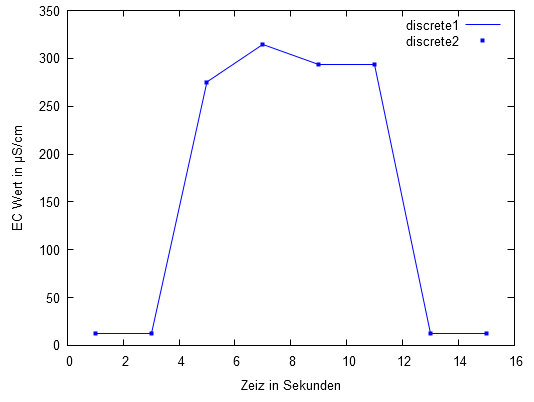
\includegraphics[height=3.25in]{ec_tests}}
\end{minipage}

\newpage
\section{Art der Daten\"ubermittlung}

\section{Datenbankmanagementsystem}

\subsection{Evaluierung RDBMS vs. NoSQL}

\subsubsection{Einleitung}
Zur Speicherung der Sensordaten soll ein geeignetes Datenbankmanagement-\\ system verwendet werden. Zu Beginn wird evaluiert, ob ein relationales oder ein NoSQL-Datenbanksystem verwendet wird. Dabei werden die jeweiligen Vor-und Nachteile von SQL und NoSQL Datenbanken aufgelistet. Besonders wert gelegt wird auf die Performance, die Konsistenz sowie dem einfachen Zugriff auf die Daten.

\subsubsection{Kriterien}

\begin{itemize}
	\item Performance: \\Gibt an, wie schnell die Lese- und Schreibleistung ist.
	\item Konsistenz: \\Gibt an, wie gut das DBMS Ma{\ss}nahmen zur Konsistenzerhaltung umsetzt.
	\item einfacher Zugriff auf Daten: \\Gibt an, wie Umfangreich die API des DBMS ist. 
\end{itemize}

\subsubsection{Optionen}

\paragraph{SQl-Datenbanken}

\textbf{Abfragesprache}\\\\
Die Abfragesprache SQL wir auf die drei Teile DDL(Data Definition Language),
DML(Data Manipulation Language) und DCL (Data Control Language) aufgeteilt.

\begin{itemize}
	\item DDL:\\ ist die Sprache f\"ur das Anlegen, \"Andern und L\"oschen von Datenstrukturen.
	\item DML:\\ ist die Sprache f\"ur das Abfragen, Einf\"ugen, \"Andern oder L\"oschen von Nutzdaten.
	\item DCL:\\ ist die Sprache f\"ur die Zugriffskontrolle.
\end{itemize}
\textbf{Konsistenz}\\\\
SQL-Datenbanken verwenden das ACID Prinzip, daher besitzen sie eine bessere Konsistenz als
NoSQL-Datenbanken. NoSQL Datenbanken verwenden das BASE Prinzip, die Daten hier sind daher 
nur "schlussendlich" konsistent. Dadurch kann es passieren das nach einem Update nicht immer 
die selben Werte zur\"uckgeliefert werden.

\paragraph{NoSQl-Datenbanken}
NoSQL-Datenbanken besitzen wegen ihres einfachen Schemas eine hohe Skalierbarkeit, welche trotz eines
hohen Datenvolumens gew\"ahrt wird. 

\subsubsection{Fazit}
SQL-Datenbanken weisen eine bessere Konsistenz auf, jedoch besitzen NoSQL-Datenbanken
eine bessere Performance und Skalierbarkeit. Da wir besonderen Wert auf die Performance
legen, haben wir uns entschieden eine NoSQL-Datenbank zu verwenden.

\subsection{Evaluierung eines NoSQL Datenbanksystems}

\subsubsection{Einleitung}
Die Folgenden Datebankmanagementsysteme wurden evaluiert:

\begin{itemize}
	\item MongoDB
	\item Redis
\end{itemize}

\subsubsection{Kriterien}

\begin{itemize}
	\item Performance: \\Gibt an, wie schnell die Lese- und Schreibleistung ist.
	\item einfacher Zugriff auf Daten: \\Gibt an, wie Umfangreich die API des DBMS ist. 
	\item Dokumentation:\\ Gibt an, wie gut das DBMS dokumentiert ist.
	\item Verbreitung:\\ Gibt an, wie weit das DBMS verbreitet ist.
\end{itemize}

\subsubsection{Optionen}

\paragraph{MongoDB}
MongoDB ist eine Schema-freie, dokumentenorientierte NoSQL-Datenbank, die in der Programmiersprache C++ geschrieben ist. Da die Datenbank dokumentenorientiert ist, kann sie Sammlungen von JSON-\"ahnlichen Dokumenten verwalten. So k\"onnen viele Anwendungen Daten auf nat\"urlichere Weise modellieren, da die Daten zwar in komplexen Hierarchien verschachtelt werden k\"onnen, dabei aber immer abfragbar und indizierbar bleiben.\\\\
Au{\ss}erdem ist MongoDB eine Allzweckdatenbank mit offenem Quellcode (OpenSource).
Sie hat u.a. folgende Merkmale:

\begin{itemize}
	\item Dokumentdatenmodell mit dynamischen Schemata
	\item Umfassende, flexible Indexunterst\"utzung
	\item Aggregation-Framework und MapReduce
	\item Auto-Sharding f\"ur horizontale Skalierbarkeit
	\item Eingebaute Replikation f\"ur Hochverf\"ugbarkeit
	\item Textsuche
	\item Erweiterte Sicherheit (z.B. Kerberos Unterst\"utzung)
	\item Speicherung gro{\ss}er Dateien mit GridFS
\end{itemize}

\paragraph{Redis}
Redis ist eine In-Memory-Datenbank mit einer einfachen Schl\"ussel-Werte-Datenstruktur. Nach einer Erhebung von DB-Engines.com ist Redis der verbreitetste Schl\"ussel-Werte-Speicher.\\
Die einfache Struktur der Datenbank eignet sich weniger f\"ur komplexe Datenstrukturen, die \"uberwiegend in der Datenbank selbst abgebildet werden soll, daf\"ur ist der gro{\ss}e Vorteil von Redis, dass es schneller ist als relationale Datenbanken wie z.B. MySQL. Bis zu ca. 100.000 Schreibvorg\"ange und ca. 80.000 Lesevorg\"ange pro Sekunde sind auf herk\"ommlicher Hardware m\"oglich.\\
Redis bietet Persistenz durch automatisiertes regelm\"a{\ss}iges Abspeichern oder per Protokolldatei, wodurch bei entsprechender Konfiguration auch eine ACID-konforme Dauerhaftigkeit erreichbar ist.

\subsubsection{Fazit}
Redis schneidet bei den Kriterien, wie z.B. der Performance und den einfachen Zugriff auf Daten durch
seine Kompaktheit, besser als MongoDB ab, hat jedoch den großen Nachteil, dass es bei serverseitiger Verwendung, extrem viel Arbeitsspeicher verbraucht, wenn einige Aquaponik Systeme ihre Daten über den Server persistieren.

\subsection{Gesamtfazit}
Es müssen sowohl auf dem lokalen Raspberry Pi, als auch auf dem Server Echtzeitdaten vorhanden sein, um einerseits auf dem Touchdisplay eine Übersicht anzuzeigen und andererseits über den Browser alle Daten zu betrachten. Da auf dem Raspberry Pi allerdings nicht viel Speicherplatz vorhanden ist, wird dafür Redis verwendet und für die serverseitige Persistierung MongoDB.


\section{Web Framework}
Bei Web Frameworks, werden durch vordefinierte und vorgefertigte Klassen, h\"aufig gebrauchte Funktionen wie Mailversand, sichere Authentifizierung, Sicherheitsfunktionen, Lokalisierung, Performance (z.B. HTTP Caching) oder grundlegende Funktionen f\"ur Webformulare vereinfacht. \\
Web Frameworks sind darauf ausgelegt, sehr schnell Ergebnisse zu erzielen und lauff\"ahige Webanwendungen zu erstellen. Dazu bieten sie einen Datenbankzugriff, Templating-Mechanismen, eine saubere Trennung von Pr\"asen-tation und Code durch Verwendung des Model-View-Controllers. \\
Da eine eigenst\"andige Implementierung all dieser Mechanismen den Arbeitsaufwand \"ubersteigen w\"urde, ist eine Verwendung eines solchen Web Frameworks unabdinglich. Welches Framework dabei gew\"ahlt wird h\"angt von folgenden Komponenten ab:
\begin{itemize}
\item Schwierigkeitsgrad
\item Lernkurve
\item Sicherheit
\item Core Library
\item Dokumentation
\end{itemize}
\subsection{Django}

\subsection{Node JS}
\subsection{Laravel}
\end{document}
